\documentclass[10pt, landscape]{article}
\usepackage[scaled=0.92]{helvet}
\usepackage{calc}
\usepackage{multicol}
\usepackage[a4paper,margin=3mm,landscape]{geometry}
\usepackage{amsmath,amsthm,amsfonts,amssymb}
\usepackage{color,graphicx,overpic}
\usepackage{hyperref}
\usepackage{newtxtext} 
\usepackage{enumitem}
\usepackage[table]{xcolor}
\usepackage{mathtools}
\setlist{nosep}
% for including images
\graphicspath{ {./images/} }

\pdfinfo{
  /Title (springboot.pdf)
  /Creator (TeX)
  /Producer (pdfTeX 1.40.0)
  /Author (Tan Ping Zhi)
  /Subject (CS2102)
/Keywords (springboot, nus,cheatsheet,pdf)}

% Turn off header and footer
\pagestyle{empty}

% redefine section commands to use less space
\makeatletter
\renewcommand{\section}{\@startsection{section}{1}{0mm}%
  {-1ex plus -.5ex minus -.2ex}%
  {0.5ex plus .2ex}%x
{\normalfont\large\bfseries}}
\renewcommand{\subsection}{\@startsection{subsection}{2}{0mm}%
  {-1explus -.5ex minus -.2ex}%
  {0.5ex plus .2ex}%
{\normalfont\normalsize\bfseries}}
\renewcommand{\subsubsection}{\@startsection{subsubsection}{3}{0mm}%
  {-1ex plus -.5ex minus -.2ex}%
  {1ex plus .2ex}%
{\normalfont\small\bfseries}}%
\makeatother

\renewcommand{\familydefault}{\sfdefault}
\renewcommand\rmdefault{\sfdefault}
%  makes nested numbering (e.g. 1.1.1, 1.1.2, etc)
\renewcommand{\labelenumii}{\theenumii}
\renewcommand{\theenumii}{\theenumi.\arabic{enumii}.}
\renewcommand\labelitemii{•}
\renewcommand\labelitemiii{•}

\definecolor{mathblue}{cmyk}{1,.72,0,.38}
\everymath\expandafter{\the\everymath \color{mathblue}}

% Don't print section numbers
\setcounter{secnumdepth}{0}

\setlength{\parindent}{0pt}
\setlength{\parskip}{0pt plus 0.5ex}
%% adjust spacing for all itemize/enumerate
\setlength{\leftmargini}{0.5cm}
\setlength{\leftmarginii}{0.5cm}
\setlist[itemize,1]{leftmargin=2mm,labelindent=1mm,labelsep=1mm}
\setlist[itemize,2]{leftmargin=4mm,labelindent=1mm,labelsep=1mm}
\setlist[itemize,3]{leftmargin=4mm,labelindent=1mm,labelsep=1mm}

% adding my commands
% tightcenter
\newenvironment{tightcenter}{%
  \setlength\topsep{0pt}
  \setlength\parskip{0pt}
  \begin{center}
    }{%
  \end{center}
}

% boxed
\newenvironment{tightbox}{%
  \setlength\topsep{0pt}
  \setlength\parskip{0pt}
  \begin{center}
    \begin{tabular}{|@{\hspace{\dimexpr\fboxsep+0.5\arrayrulewidth}}c@{\hspace{\dimexpr\fboxsep+0.5\arrayrulewidth}}|}
      \hline
    }
    {%
    \\ \hline
    \end{tabular}
  \end{center}
}

% fixed width box
\newenvironment{fixedbox}[1][0.7]{
  \setlength\topsep{0pt}
  \setlength\parskip{0pt}
  \begin{center}
    \begin{tabular}{|>{\centering\arraybackslash}m{#1\linewidth}|}
    \hline
  }{
  \\ \hline
  \end{tabular}
  \end{center}
}

% definition of a new term
\usepackage{soul}
\definecolor{paleyellow}{RGB}{251,243,218}
\newcommand{\definition}[2][]{\sethlcolor{paleyellow}\hl{\textbf{#2}} #1  $\rightarrow$}
% inline definition
\newcommand{\ildefinition}[1]{\sethlcolor{paleyellow}\hl{\textbf{#1}}}

% important note (attention)
\newcommand{\attention}{{\color{red}\textbf{! }}}

% nice proof
\newenvironment{niceproof}[1][Proof]
{%
  \sbox0{\textit{#1}. }%
  \list{}{\labelwidth\wd0 \leftmargin\wd0 \labelsep 0pt }
\item[\usebox0]}
  {\endlist}


\usepackage{color, soul}
\usepackage{listings}
\usepackage{inconsolata}

\definecolor{codegreen}{rgb}{0,0.6,0}
\definecolor{codegray}{rgb}{0.5,0.5,0.5}
\definecolor{codepurple}{HTML}{C42043}
\definecolor{backcolour}{HTML}{F2F2F2}
\definecolor{bookColor}{cmyk}{0,0,0,0.90}

\newcommand{\code}[1]{\texttt{\sethlcolor{backcolour}\hl{$\,$#1$\,$}}}

% SQL code blocks
% define SQL styles
\lstdefinestyle{mySQL}{%
  language=SQL,
  backgroundcolor=\color{backcolour},
  commentstyle=\color{codegreen},
  keywordstyle=\color{codepurple},
  numberstyle=\numberstyle,
  stringstyle=\color{codepurple},
  basicstyle=\scriptsize\ttfamily,
  breaklines=true,
}

\DeclareMathOperator{\pairwisemax}{pairwise-max}

% -----------------------------------------------------------------------

\begin{document}
\raggedright
\footnotesize
\begin{multicols*}{2}
  % multicol parameters
  \setlength{\columnseprule}{0.25pt}

  \begin{center}
    \fbox{%
    \parbox{0.8\linewidth}{\centering \textcolor{black}{
      {\Large\textbf{Spring Boot}}
      \\ \normalsize{CSIT 2024}}
    \\ {\footnotesize \textcolor{gray}{github/TanPingZhi}}
    }%
    }
  \end{center}

  \section{Spring Boot architecture}
  \begin{itemize}
    \item Presentation
    \begin{itemize}
      \item Authentication
      \item JSON translation
    \end{itemize}
    \item Business
    \begin{itemize}
      \item business logic
      \item validation
      \item authorization
    \end{itemize}
    


  \section{Lombok}
  references: \url{https://projectlombok.org/features/constructor}


  \verb|@NoArgsConstructor|
  \begin{itemize}
    \item Generates a no-args constructor. eg. \verb|Person() {}|
  \end{itemize}
  \verb|@RequiredArgsConstructor|
  \begin{itemize}
    \item Generates a constructor for all final and not null fields, with parameter order same as field order.
  \end{itemize}
  \verb|@AllArgsConstructor|
  \begin{itemize}
    \item Generates a constructor for all fields.
  \end{itemize}

  \section{Spring Repository}
  \textbf{Purpose}
  \begin{itemize}
    \item Encapsulates data access logic, make it easier to do CRUD
  \end{itemize}
  \textbf{Interface}
  \begin{itemize}
    \item \verb|CrudRepository<T, ID>|
    \item \verb|PagingAndSortingRepository<T, ID>|
    \item \verb|JpaRepository<T, ID>|
  \end{itemize}
  \textbf{Methods}
  \begin{itemize}
    \item \verb|save(S entity)|
    \item \verb|findById(ID primaryKey)|
    \item \verb|findAll()|
    \item \verb|deleteById(ID primaryKey)|
  \end{itemize}

  \subsection{Example Usage}
  \begin{verbatim}
import org.springframework.data.repository.CrudRepository;
@Repository
public interface PersonRepository extends CrudRepository<Person, Long> {
  // custom queries
}
\end{verbatim}
  \textbf{Usage in Service}
  \begin{verbatim}
@Service
public class PersonService {
  @Autowired
  private PersonRepository personRepository;
  public Person savePerson(Person person) {
    return personRepository.save(person);
  }
  // other methods
}
\end{verbatim}


  \section{Database layers}
  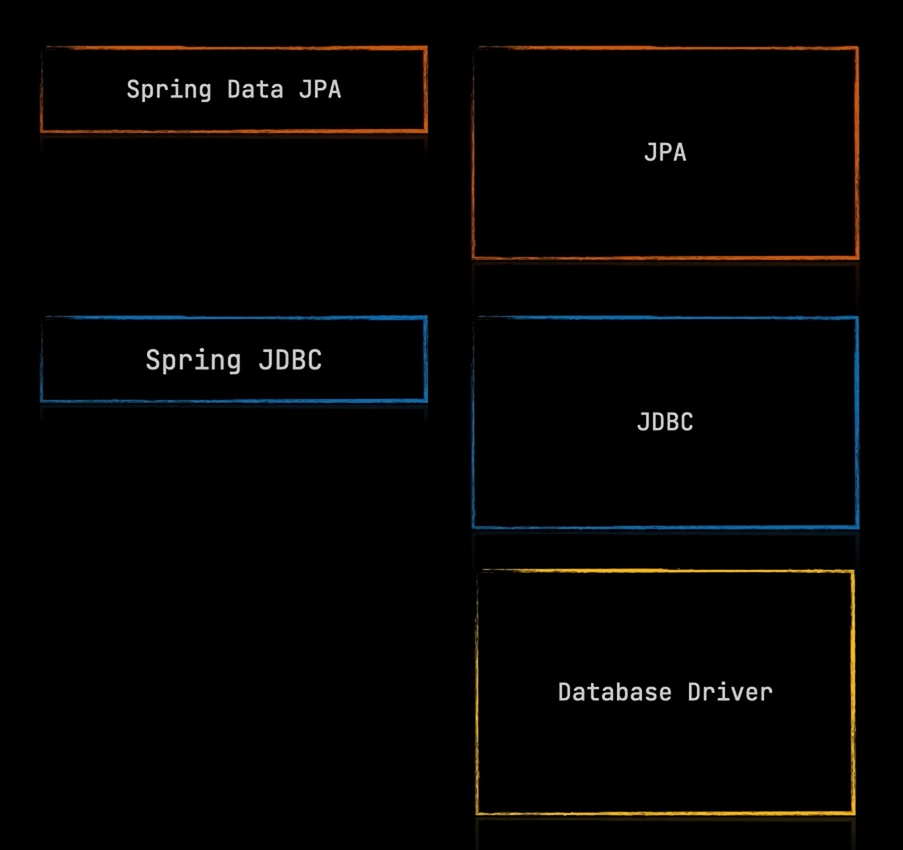
\includegraphics[width=\linewidth/2]{databaselayers.png}

  \subsection{Database drivers}
  \begin{itemize}
    \item Allows you to interact with the database from the Java code
  \end{itemize}
  \subsection{JDBC: Java Database Connectivity}
  \begin{itemize}
    \item Allows developers to use custom SQL queries
    \item Have to handle mapping to Java objects manually
  \end{itemize}

  \subsection{Spring JDBC}
  \begin{itemize}
    \item Builds on top of JDBC
    \item Provides the JDBC template
    \item Makes interacting with the database with SQL easier
  \end{itemize}

  \subsection{JPA: Java Persistence API}
  \begin{itemize}
    \item Allows interaction with the database using Java objects
    \item Handles all the generation of the sql and the mapping to and from Java objects
    \item Builds on top of JDBC
  \end{itemize}

  \subsection{Spring Data JPA}
  \begin{itemize}
    \item Repository
    \item Hibernate is a ORM (Object Relational Mapping) framework
  \end{itemize}

  \section{Connect to a H2 Database}
  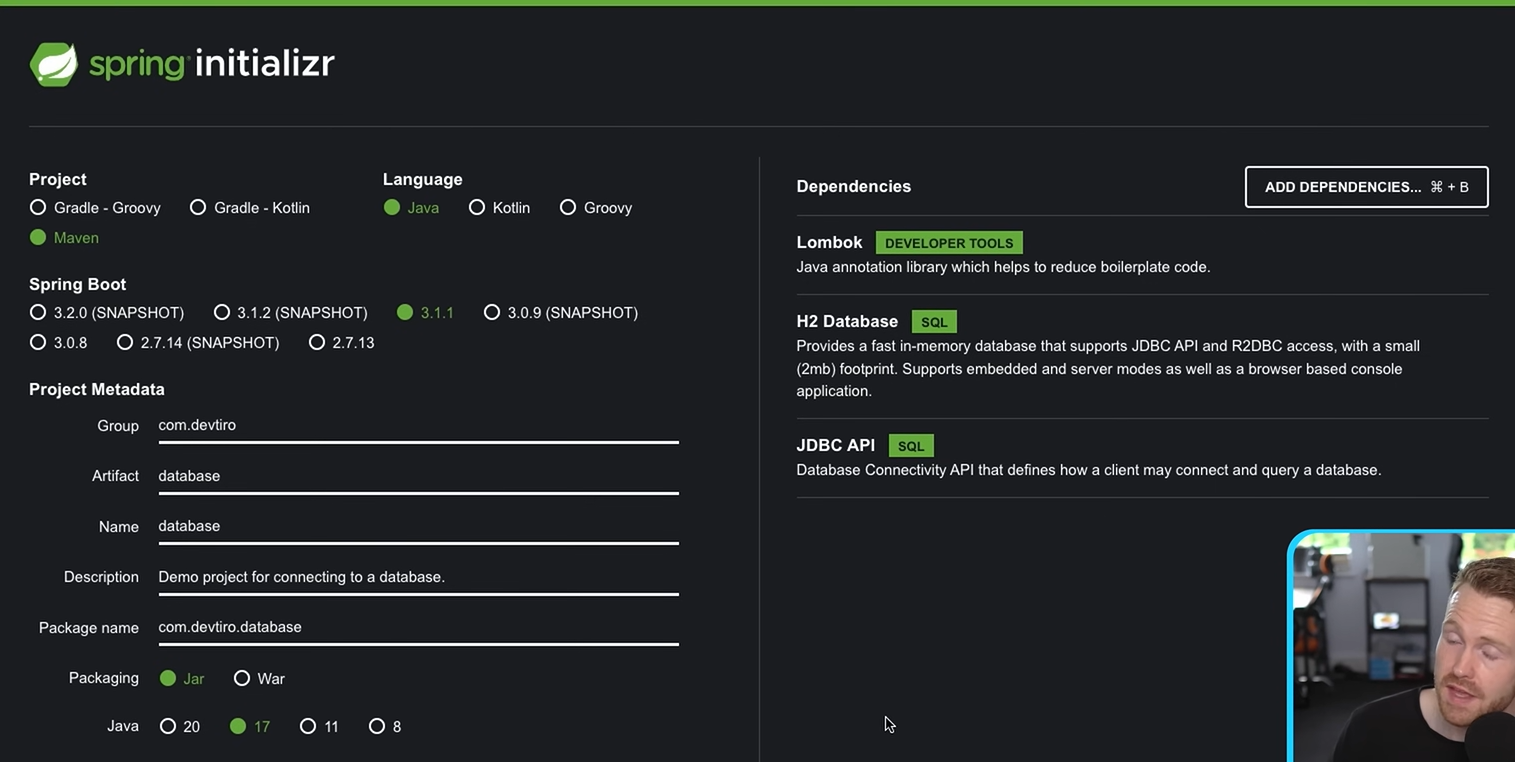
\includegraphics[width=\linewidth/2]{downloadh2.png}

  \begin{verbatim}
package com.pingzhi.database;
import lombok.extern.java.Log;
import org.springframework.boot.CommandLineRunner;
import org.springframework.boot.SpringApplication;
import org.springframework.boot.autoconfigure.SpringBootApplication;
import org.springframework.jdbc.core.JdbcTemplate;
import javax.sql.DataSource;

@Log
@SpringBootApplication
public class DatabaseApplication implements CommandLineRunner {
  private final DataSource dataSource;
  public DatabaseApplication(final DataSource datasource) {
    this.dataSource = datasource;
  }
  public static void main(String[] args) {
    SpringApplication.run(DatabaseApplication.class, args);
  }
	@Override
	public void run(final String... args) {
		log.info("Datasource: " + dataSource.toString());
		final JdbcTemplate jdbcTemplate = new JdbcTemplate(dataSource);
		jdbcTemplate.execute("select 1");
	}
}
\end{verbatim}
  \begin{itemize}
    \item \hl{SpringApplication.run(...) is the driver to the Spring Boot application}
    \item \hl{mistake in the tutorial: should use "jdbcTemplate" instead of "restTemplate"}
  \end{itemize}


  \section{Introduction to DAO: Data Access Object pattern}
  Consider book and auther entities
  \begin{itemize}
    \item Book has 1 Author
    \item Author has $\ge 1$ Book
  \end{itemize}

  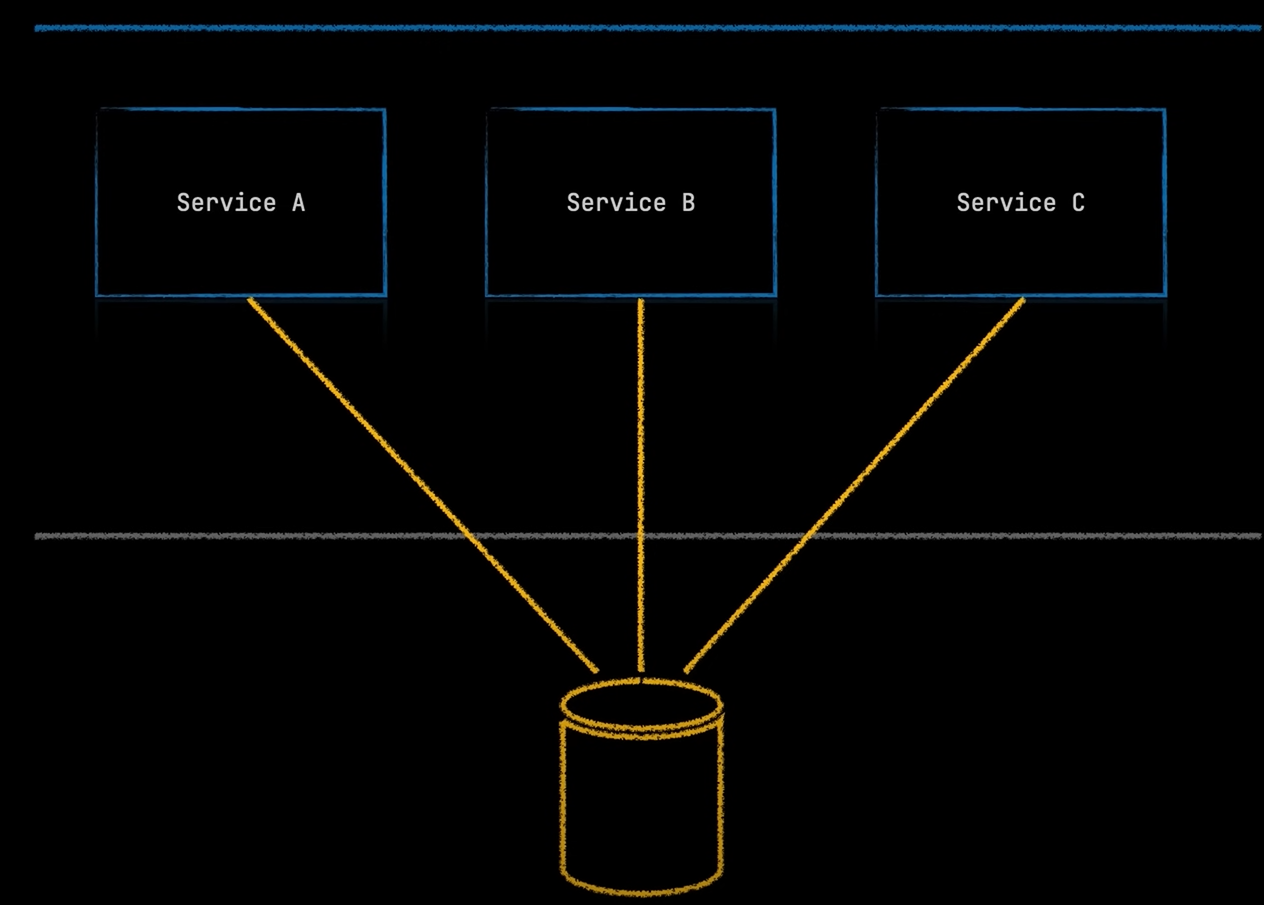
\includegraphics[width=\linewidth/2]{originalnodao.png}
  \begin{itemize}
    \item Lets say that we have 3 services that need to interact with the database.
    \item If we use jdbc, each services will need to convert between sql and java objects and will result in duplicate code.
  \end{itemize}
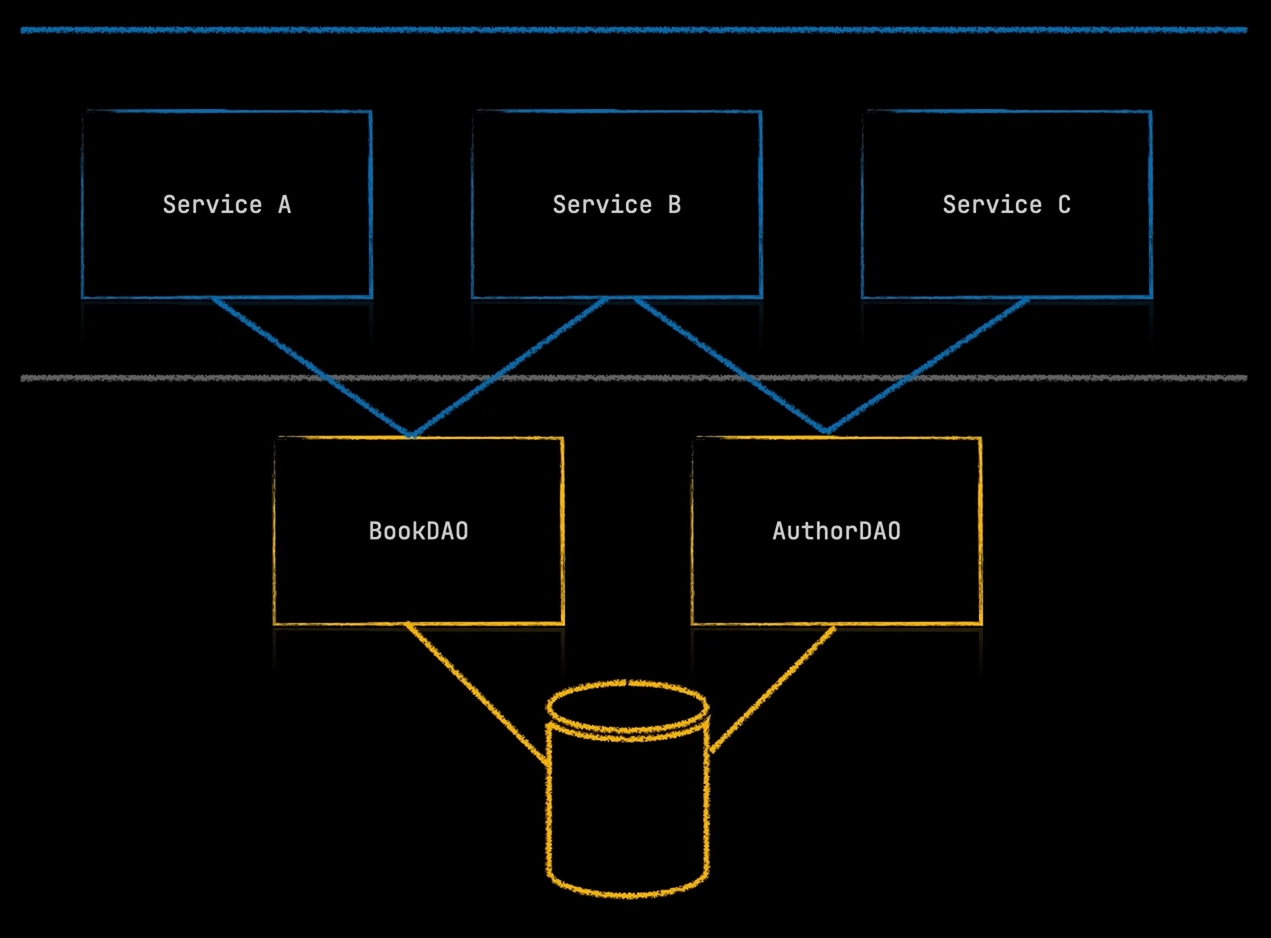
\includegraphics[width=\linewidth/2]{dao.png}
\begin{itemize}
  \item Abstracts the conversion between sql and java objects into a single class
\end{itemize}
\subsection{Author Domain}
\begin{verbatim}
package com.devtiro.database.domain;
import lombok.AllArgsConstructor;
import lombok.Builder;
import lombok.Data;
import lombok.NoArgsConstructor;
@Data
@AllArgsConstructor
@NoArgsConstructor
@Builder
public class Author {
  private Long id;
  private String name;
  private Integer age;
}
\end{verbatim}
\begin{itemize}
  \item \hl{@Data: a Lombok annotation that generates getters, setters, equals, hashcode, and toString}
  \item \hl{@Builder: builder pattern}
  \item \hl{Long id: so that it can be null instead of 0}
\end{itemize}

\subsection{Book Domain}
\begin{verbatim}
// same as Author
public class Book {
  private String isbn;
  private String title;
  private Long authorId;
}
\end{verbatim}
\subsection{File structure}
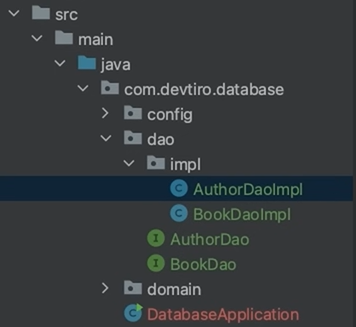
\includegraphics[width=\linewidth/2]{filestructure7_3.png}
\subsection{Author DAO}
\begin{verbatim}
package com.devtiro.database.dao.impl;
import com.devtiro.database.dao.AuthorDao;
import org.springframework.jdbc.core.JdbcTemplate;
public class AuthorDaoImpl implements AuthorDao {
    private final JdbcTemplate jdbcTemplate;
    public AuthorDaoImpl(final JdbcTemplate jdbcTemplate) {
        this.jdbcTemplate = jdbcTemplate;
    }
}
\end{verbatim}
\begin{itemize}
  \item \hl{allows us to inject the JdbcTemplate into the AuthorDaoImpl}
\end{itemize}

\subsection{Book DAO}
\begin{itemize}
  \item Similar to Author Dao
\end{itemize}

\section{Create DAO}
\begin{verbatim}
public class AuthorDaoImpl implements AuthorDao {
  // ... continuing from previous snippet
  @Override
  public void create(Author author) {
      jdbcTemplate.update(
              "INSERT INTO authors (id, name, age) VALUES (?, ?, ?)",
              author.getId(), author.getName(), author.getAge()
      );
  }
}
\end{verbatim}

\section{Test Auther DAO}
\begin{verbatim}
@ExtendWith(MockitoExtension.class)
public class AuthorDaoImplTests {
    @Mock
    private JdbcTemplate jdbcTemplate;
    @InjectMocks
    private AuthorDaoImpl underTest;
    @Test
    public void testThatCreateAuthorGeneratesCorrectSql() {
        Author author = Author.builder()
                .id(1L)
                .name("Abigail Rose")
                .age(80)
                .build();
        underTest.create(author);
        verify(jdbcTemplate).update(
                eq("INSERT INTO authors (id, name, age) VALUES (?, ?, ?)"),
                eq(1L), eq("Abigail Rose"), eq(80)
        );
    }
}
\end{verbatim}
\begin{itemize}
  \item \hl{Author.builder() allows us to create an Author object}
\end{itemize}

\section{10.1 REST API Design}
We will be putting books and authors in a postgres db
\textbf{RestController}
\begin{itemize}
  \item Primarily designed for server-server communication and RESTful APIs
  \item Not meant for rendering content in a browser
  \item Good for distributed systems
\end{itemize}
\subsection{10.2 Author Create Endpoint}


\end{multicols*}
\end{document}
